
% Language: english, slovak
% Document type: article (bachelor thesis), report (master thesis)
%%
%% CHECK THE PLACE WITH "!!!!"
%%

%%
%% !!!! select one for BACHELOR THESIS
%%
%\documentclass[a4paper,english,12pt,appendix]{article}
%\documentclass[a4paper,slovak,12pt,appendix]{article}
%\documentclass[a4paper,slovak,12pt]{article}

%%
%% !!!! select one for MASTER THESIS
%%
%\documentclass[a4paper,english,12pt,appendix]{report}
\documentclass[a4paper,slovak,12pt,appendix]{report}

\usepackage{ifthen}
\newboolean{english}
\newboolean{bachelor}

%%
%% !!!! for MASTER THESIS set to FALSE
%%
\setboolean{bachelor}{false}

%%
%% !!!! for SLOVAK VERSION set to FALSE
%%
\setboolean{english}{false}



%%
%% Formats and Defs
%%
%!TEX root = main.tex

% Packages
\usepackage{epsf}
\usepackage{epsfig}
\usepackage[T1]{fontenc}
\usepackage{latexsym}
\usepackage{ucs}
\usepackage[utf8x]{inputenc}
\usepackage{float}
\usepackage[usenames]{color}
\usepackage{newcent}
\usepackage{graphicx}
\usepackage{setspace}
\onehalfspacing
\usepackage[numbers]{natbib}
\usepackage{setspace}
\usepackage{url}
\usepackage{eso-pic}
\usepackage{listings}
\usepackage{verbatim}
\usepackage[table,xcdraw]{xcolor}
\usepackage{moreverb}
\usepackage{microtype}
%\usepackage{fixltx2e}
\usepackage[noauto]{chappg}
\usepackage{lmodern}
\usepackage{appendix}
\usepackage{libertine}
\usepackage{array}
\usepackage{changepage}
\usepackage{setspace}
\usepackage{afterpage}
\usepackage{pdfpages}

\newcommand\blankpage{%
    \null
    \thispagestyle{empty}%
    \addtocounter{page}{-1}%
    \newpage}

%\usepackage{showframe}
\usepackage[margin=1in]{geometry}

% Language
\ifthenelse {\boolean{english}}
{
	\usepackage[english]{babel}

	\renewcommand{\lstlistingname}{Example}
	\renewcommand{\lstlistlistingname}{List of Examples}
}
{
	\usepackage[slovak]{babel}
	\usepackage[IL2]{fontenc}

	\renewcommand{\lstlistingname}{Ukážka}
	\renewcommand{\lstlistlistingname}{Zoznam ukážok}
}


% Bookmarks

% black references
%\usepackage[pdfborder={0 0 0}]{hyperref}

% red references
\usepackage[colorlinks=true,allcolors = black]{hyperref}

% Colors
\definecolor{light-gray}{gray}{0.95}
\definecolor{gray}{gray}{0.2}
\definecolor{blue}{rgb}{0,0,1}
\definecolor{red}{rgb}{1,0,0}
\definecolor{green}{rgb}{0,0.69,0}
\definecolor{yellow}{rgb}{1,0.35,0}

% Listings settings
\lstdefinelanguage{lua}{
	morekeywords={and,break,do,else,elseif,end,false,for,function,if,in,local,nil,not,or,repeat,return,then,true,until,while},
	morekeywords={[2]arg,assert,collectgarbage,dofile,error,_G,getfenv,getmetatable,ipairs,load,loadfile,loadstring,next,pairs,pcall,print,rawequal,rawget,rawset,select,setfenv,setmetatable,tonumber,tostring,type,unpack,_VERSION,xpcall},
	morekeywords={[2]coroutine.create,coroutine.resume,coroutine.running,coroutine.status,coroutine.wrap,coroutine.yield},
	morekeywords={[2]module,require,package.cpath,package.load,package.loaded,package.loaders,package.loadlib,package.path,package.preload,package.seeall},
	morekeywords={[2]string.byte,string.char,string.dump,string.find,string.format,string.gmatch,string.gsub,string.len,string.lower,string.match,string.rep,string.reverse,string.sub,string.upper},
	morekeywords={[2]table.concat,table.insert,table.maxn,table.remove,	table.sort},
	morekeywords={[2]math.abs,math.acos,math.asin,math.atan,math.atan2,math.ceil,math.cos,math.cosh,math.deg,math.exp,math.floor,math.fmod,math.frexp,math.huge,math.ldexp,math.log,math.log10,math.max,math.min,math.modf,math.pi,math.pow,math.rad,math.random,math.randomseed,math.sin,math.sinh,math.sqrt,math.tan,math.tanh},
	morekeywords={[2]io.close,io.flush,io.input,io.lines,io.open,io.output,io.popen,io.read,io.tmpfile,io.type,io.write,file:close,file:flush,file:lines,file:read,file:seek,file:setvbuf,file:write},
	morekeywords={[2]os.clock,os.date,os.difftime,os.execute,os.exit,os.getenv,os.remove,os.rename,os.setlocale,os.time,os.tmpname},
	keywordstyle=\color{blue}\normalfont,
	ndkeywordstyle=\color{black}\normalfont,
	commentstyle=\color{red}\ttfamily,
	stringstyle=\color{green}\ttfamily,
	identifierstyle=\color{gray},
	sensitive=true,
	morecomment=[l]{--},
	morecomment=[s]{--[[}{]]--},
	morestring=[b]",
	morestring=[d]',
	backgroundcolor=\color{white},
	frame=single,
	frameround=ffff,
	captionpos=b,
	basicstyle=\scriptsize
}

\lstdefinelanguage{nil}{
  identifierstyle=\color{black},
  sensitive=false,
  columns=flexible,
  backgroundcolor=\color{white},
  frameround=ffff,
  captionpos=b
}

\lstdefinelanguage{javascript}{
  keywords={typeof, new, true, false, catch, function, return, null, catch, switch, var, if, in, while, do, else, case, break},
  ndkeywords={class, export, boolean, throw, implements, import, this},
  sensitive=false,
  comment=[l]{//},
  morecomment=[s]{/*}{*/},
  morestring=[b]',
  morestring=[b]",
  keywordstyle=\color{blue}\normalfont,
	ndkeywordstyle=\color{black}\normalfont,
	commentstyle=\color{red}\ttfamily,
	stringstyle=\color{green}\ttfamily,
	identifierstyle=\color{gray},
	backgroundcolor=\color{white},
	frame=single,
	frameround=ffff,
	captionpos=b,
	basicstyle=\scriptsize
}

\lstdefinestyle{color}
	{identifierstyle=\color{green}\bfseries, commentstyle=\color{yellow}\bfseries, stringstyle=\color{blue}, keywordstyle=\color{red}\bfseries,morecomment=[l]{\#}}

\lstset{postbreak=\small>>\space,prebreak=\small>>,breakindent=13pt,breaklines=true,inputencoding=utf8x,tabsize=2,showtabs=false,tab=$\to$,style=color,basicstyle=\footnotesize\ttfamily\normalfonts,frame=lines,frameround=tttt}

% Figures settings
\usepackage[small,normal,up]{caption2}
\renewcommand{\captionfont}{\small\itshape}
\graphicspath{{figures/}}

%
% this makes list spacing much better.
%
\newenvironment{my_itemize}{
\begin{itemize}
  \setlength{\itemsep}{1pt}
  \setlength{\parskip}{0pt}
  \setlength{\parsep}{0pt}}{
\end{itemize}
}

\newenvironment{my_enumerate}{
\begin{enumerate}
  \setlength{\itemsep}{1pt}
  \setlength{\parskip}{0pt}
  \setlength{\parsep}{0pt}}{
\end{enumerate}
}

\newcommand{\emptyitem}{\item[]}
\newcommand{\myitem}{\item[$-$]}

%Font settings
\makeatletter
\renewcommand{\paragraph}{\@startsection{paragraph}{4}
{0ex}%
{-3.25ex plus -1ex minus -0.2ex}%
{1.5ex minus 0.2ex}%
 {\normalfont\normalsize\bfseries}}

\makeatother


\stepcounter{secnumdepth}
\stepcounter{tocdepth}

\setcounter{secnumdepth}{3}
\setcounter{tocdepth}{3}


% Section rules
\usepackage{sectsty}
\usepackage{times}
\allsectionsfont{\normalfont\sffamily\bfseries}

% Paragraph format
\setlength{\parindent}{0em}
\setlength{\parskip}{1em}

% Chapter formatting
\usepackage{titlesec}

\titleformat{\chapter}
  {\normalfont\sffamily\LARGE\bfseries}{\thechapter}{1em}{}[{\titlerule[0.5pt]}]
\titlespacing*{\chapter}{0pt}{0ex}{2.5ex}


%%%%%%%%%%%%%%%%%%%%%%%%%%%%%%%%%%%%%%%%%%%%%%%%%%%%%%%%%%%%%%%%%%%%%%%%%%%%%%%%%%%%%%%%

%% !!!! set your own definitions

%-------definitions-----
\newcommand{\Author}{Bc. Martin Šrank}
\newcommand{\Title}{Podpora diverzity a~aktuálnosti informačných bulletinov v~systéme pre~odpovedanie na~otázky}
\newcommand{\Supervisor}{Ing. Ivan Srba, PhD.}
\newcommand{\Place}{Ústav informatiky, informačných systémov a softvérového inžinierstva, FIIT STU, Bratislava}
\newcommand{\Year}{2018}
\newcommand{\Month}{Máj }
\newcommand{\FIIT}{FIIT-5208-72397}
\newcommand{\Field}{9.2.6 Informačné systémy}
\newcommand{\Program}{Informačné systémy}
\newcommand{\AuthorEN}{Martin Šrank}
\newcommand{\TitleEN}{Improving Diversity and~Freshness of~Newsletters in~Community Question Answering Systems}
\newcommand{\SupervisorEN}{Dr. Ivan Srba}
\newcommand{\ProgramEN}{Information Systems}
\newcommand{\MonthEN}{May }

%%
%% DON'T TOUCH
%%
%% PDF meta-data
\hypersetup{%
pdftitle={\Title},%
pdfauthor={\Author},%
pdfkeywords={key words},%
}%

%%%%%%%%%%%%%%%%%%%%%%%%%%%%%%%%%%%%%%%%%%%%%%%%%%%%%%%%%%%%%%%%%%%%%%%%%%%%%%%%%%%%%%%%
\begin{document}

%%
%% Title Page
%%
%!TEX root = main.tex
\begin{center}
\thispagestyle{empty}
\ifthenelse {\boolean{english}}
{
	{\Large Slovak University of Technology in Bratislava}\textbf{}\\
	{\Large Faculty of Informatics and Information Technologies}\textbf{}\\[\baselineskip]
}
{
	{\Large Slovenská technická univerzita v Bratislave}\textbf{}\\
	{\Large Fakulta informatiky a informačných technológií}\textbf{}\\[\baselineskip]
}
{\large \FIIT}\\
\vspace*{7cm}
{\Large \Author}\textbf{}\\[\baselineskip]
{\Large \Title}\textbf{}\\[\baselineskip]
\ifthenelse {\boolean{english}}
{
	\ifthenelse {\boolean{bachelor}}
	{
		{\large Bachelor thesis}\\
	}
	{
		{\large Master thesis}\\
	}
}
{
	\ifthenelse {\boolean{bachelor}}
	{
		{\large Bakalárska práca}\\
	}
	{
		{\large Diplomová práca}\\
	}
}

\end{center}
\vspace*{7cm}
\ifthenelse {\boolean{english}}
{
	Supervisor: \Supervisor \\\\
}
{
	Vedúci práce: \Supervisor \\\\
}
\Month \Year
\newpage
\begin{center}
\thispagestyle{empty}
\ifthenelse {\boolean{english}}
{
	{\Large Slovak University of Technology in Bratislava}\textbf{}\\
	{\Large Faculty of Informatics and Information Technologies}\textbf{}\\[\baselineskip]
}
{
	{\Large Slovenská technická univerzita v Bratislave}\textbf{}\\
	{\Large Fakulta informatiky a informačných technológií}\textbf{}\\[\baselineskip]
}
%{\large \FIIT}\\
%\vspace*{5cm}
\vspace*{6.5cm}
{\Large \Author}\textbf{}\\[\baselineskip]
{\Large \Title}\textbf{}\\[\baselineskip]
\ifthenelse {\boolean{english}}
{
	\ifthenelse {\boolean{bachelor}}
	{
		{\large Bachelor thesis}\\
	}
	{
		{\large Master thesis}\\
	}
}
{
	\ifthenelse {\boolean{bachelor}}
	{
		{\large Bakalárska práca}\\
	}
	{
		{\large Diplomová práca}\\
	}
}
\end{center}
\vspace*{6cm}
\ifthenelse {\boolean{english}}
{
	Study program: \Program\\
	Field of Study: \Field\\
	Place: \Place\\
	Vedúci práce: \Supervisor \\\\
}
{
	Študijný program:~~~~~~~\Program\\
	Študijný odbor:~~~~~~~~~~~\Field\\
	Miesto vypracovania:~Ústav informatiky, informačných systémov a softvérového inžinierstva,\\
	\hspace*{3.8cm}FIIT STU, Bratislava\\
	Vedúci práce:~~~~~~~~~~~~~~\Supervisor \\\\
}
\Month \Year
\afterpage{\blankpage}


%%
%% Anotation
%%
\pagenumbering{roman}\setcounter{page}{2}
	\newpage
\thispagestyle{plain}
\begin{center}
\begin{Large}
\textbf{Anotácia} \\
\end{Large}
\end{center}
Slovenská technická univerzita v Bratislave \\
FAKULTA INFORMATIKY A INFORMAČNÝCH TECHNOLÓGIÍ \\
\noindent
Študijný program: \Program \\
\noindent
Autor: \Author \\
\ifthenelse {\boolean{bachelor}}
{
	{Bakalárska práca: }\Title \\
}
{
	{Diplomová práca: }\Title \\
}
Vedúci práce: \Supervisor \\
\Month \Year \\
\noindent
\\
Lorem ipsum dolor sit amet, consectetur adipisicing elit, sed do eiusmod tempor incididunt ut labore et dolore magna aliqua. Ut enim ad minim veniam, quis nostrud exercitation ullamco laboris nisi ut aliquip ex ea commodo consequat. Duis aute irure dolor in reprehenderit in voluptate velit esse cillum dolore eu fugiat nulla pariatur. Excepteur sint occaecat cupidatat non proident, sunt in culpa qui officia deserunt mollit anim id est laborum....
\newpage
\thispagestyle{plain}
\begin{center}
\begin{Large}
\textbf{Annotation} \\
\end{Large}
\end{center}
Slovak University of Technology Bratislava \\
FACULTY OF INFORMATICS AND INFORMATION TECHNOLOGIES \\
\noindent
Degree Course: \Program \\
\noindent
Author: \Author \\
\ifthenelse {\boolean{bachelor}}
{
	{Bachelor thesis: }\Title \\
}
{
	{Master thesis: }\Title \\
}
Supervisor: \Supervisor \\
\Month \Year \\
\noindent
\\
Lorem ipsum dolor sit amet, consectetur adipisicing elit, sed do eiusmod tempor incididunt ut labore et dolore magna aliqua. Ut enim ad minim veniam, quis nostrud exercitation ullamco laboris nisi ut aliquip ex ea commodo consequat. Duis aute irure dolor in reprehenderit in voluptate velit esse cillum dolore eu fugiat nulla pariatur. Excepteur sint occaecat cupidatat non proident, sunt in culpa qui officia deserunt mollit anim id est laborum....

%%
%% Declaration
%%
%!TEX root = main.tex
\newpage
\thispagestyle{plain}
\vspace*{19cm}
\begin{large}
\noindent
%\textbf{DECLARATION} \\
\textbf{ČESTNÉ PREHLÁSENIE} \\
\end{large}
\noindent
Čestne prehlasujem, že záverečnú prácu som vypracoval samostatne s~použitím uvedenej literatúry a~na základe svojich
vedomostí a~znalostí.
\vspace*{1.5cm}\\
V Bratislave, 12. 12. 2017 \hspace*{6.5cm}.....................................\\
\hspace*{11.5cm} \Author
\afterpage{\blankpage}


%%
%% Contents
%%
%\pagestyle{empty}
\newpage
\setlength{\parskip}{0em}
\tableofcontents{}
\setlength{\parskip}{1em}

%%
%% Lists
%%
% \newpage
% List of Figures
% \listoffigures
% \newpage
% List of Tables
% \listoftables
% \newpage
% List of Listings
% \lstlistoflistings


%%
%% Clear Page And Set New Page Counter
%%
\clearpage
\pagenumbering{arabic}
\setcounter{page}{1}

\ifthenelse {\boolean{bachelor}}
{
	%\sectionfont{\sectionrule{0pt}{0pt}{-2ex}{0.5pt}}
}
{
	%\sectionfont{\sectionrule{0pt}{0pt}{-2ex}{0pt}}
}

%%
%% Introduction
%%
%!TEX root = main.tex
\afterpage{\blankpage}
\newpage
\chapter{Úvod}

Informačné bulletiny (angl.~\emph{newsletters}) sú stále jednou z najčastejšie používaných foriem informovania používateľov
webových portálov o novinkách, akciách alebo zaujímavom obsahu na webe. Používatelia radi využívajú informačné bulletiny
svojich obľúbených webových portálov, pretože predstavujú jednoduchý a~prehľadný spôsob prezentácie obsahu, ktorý je navyše
doručený pohodlne priamo do používateľovej e-mailovej schránky.

Informačné bulletiny zastávajú ešte väčšiu rolu v rámci online komunít, ktoré produkujú veľké množstvo používateľmi
vytváraného obsahu. Medzi populárne druhy takýchto online komunít patria aj systémy pre odpovedanie na otázky
(angl.~\emph{Community Question Answering systems -- CQA}). Veľké množstvo obsahu, ktoré v~týchto systémoch vzniká,
si vyžaduje nasadzovanie personalizačných techník za~účelom poskytnutia relevantného obsahu používateľom.

Výskum v oblasti CQA systémov sa v súčasnosti skôr orientuje na skúmanie správania používateľov, kladenia otázok a odpovedania.
Problematike informačných bulletinov v doméne CQA systémov zatiaľ nebola venovaná dostatočná pozornosť a to napriek tomu,
že existujúce informačné bulletiny nespĺňajú očakávania komunity a sú pre ne charakterisické viaceré problémy, napr.
akým spôsobom ich vhodne personalizovať a ako zároveň zabezpečiť diverzitu ich obsahu.

Cieľom našej práce je analyzovať súčasný stav výskumu odporúčania otázok v~doméne CQA systémov a navrhnúť riešenie pre
tvorbu personalizovaných informačných bulletinov v systémoch pre odpovedanie na otázky. V našej práci sa~zameriavame
predovšetkým na skúmanie vplyvu zavedenia diverzity a podpory aktuálnosti na úspešnosť personalizovaného odporúčania
otázok vo forme informačných bulletinov.

Nasledujúca kapitola sa venuje informačným bulletinom -- čo sú to informačné bulletiny, aké je ich využitie v rôznych
systémoch a aké problémy sú s nimi spájané. Ďalšia kapitola rozoberá problematiku systémov pre odpovedanie na otázky,
opisuje ich rozdelenie a problémy a ďalej sa venuje doméne odporúčacích systémov a odporúčania v CQA systémoch.
Nasleduje kapitola opisujúca problematiku diverzity a aktuálnosti v odporúčaní.

Piata kapitola obsahuje samotný návrh riešenia personalizovaného informačného bulletinu v CQA systéme. Nasledujú kapitoly
opisujúce implementáciu navrhnutých metód a ich overenie v online nekontrolovanom experimente. Záver práce tvorí vyhodnotenie
a prílohy.


%%
%% analysis
%%
%!TEX root = main.tex

\newpage
\chapter{Informačné bulletiny}

Informačné bulletiny (angl. \emph{newsletters}) sú aj v súčasnosti jedným z najrozšírenejších spôsobov, ako v online
prostredí informovať používateľov o dianí na webovom portáli. Prevádzkovatelia webových portálov využívajú informačné
bulletiny na predstavenie nového obsahu, akciového tovaru, zaujímavostí z určitej oblasti alebo špeciálnych ponúk pre
svojich používateľov a zákazníkov. Informačné bulletiny sú tiež využívané ako prostriedok pre motiváciu používateľov
k opätovnej návšteve webového portálu.

Informačné bulletiny spravidla nadobúdajú formu e-mailu, ktorý je zvyčajne v pravidelných intervaloch doručovaný
do schránok používateľov, ktorí o jeho doručovanie prejavili záujem.


\section{Problémy informačných bulletinov}
Hlavným problémom informačných bulletinov v súčasnosi je stále sa znižujúva miera interakcie používateľov
s informačnými bulletinmi.

Štúdia spoločnosti Silverpop z roku 2012~\cite{mailmarketing} na vzorke informačných bulletinov 1124 spoločností ukázala,
že počet používateľov, ktorí vôbec otvoria informačný bulletin sa pohybuje na úrovni 20\% a stále klesá. Navyše konkrétne
v oblasti technológií sa táto hodnota pohybuje len na 16,5\%. Ešte menšia je miera preklikov
(angl. \emph{Click-through rate - CTR}), ktorá sa celkovo pohybuje na úrovni 5,4\% a v prípade technologicky zameraných
informačných bulletinov len 3,6\%. Napriek tomu sa miera odhlásení z odoberania (angl. \emph{unsubscribe rate}) pohybuje
len na úrovni 2\%.

Dôvodov, prečo používatelia prejavujú iba malý záujem o informačné bulletiny ktoré im sú doručované, môže byť niekoľko.
Jedným z takýchto dôvodov môže byť vysoká saturácia -- používateľom chodí priveľké množstvo informačných bulletinov,
dôsledkom čoho používatelia rezignujú a tieto e-maily ani neotvárajú.
Hlavným nedostatkom informačných bulletinov, a zároveň dôvodom, prečo iba 5\% používateľov klikne na obsah v informačnom
bulletine, je však relevancia ponúkaného obsahu.


\section{Relevancia v informačných bulletinoch}

Množstvo webových portálov doručuje všetkým svojim používateľom presne ten istý obsah informačného bulletinu.
Často je tento obsah vytváraný manuálne editormi, a zameriava sa len všeobecne na aktuálne dianie na danom webovom
portáli. Takýto všeobecný informačný bulletin však nutne nemôže byť dostatočne relevantný pre značnú časť používateľov.

Riešením problému relevancie infromačných bulletinov je vytváranie personalizovaných informačných bulletinov, ktoré
každému používateľovi ponúkajú len ten obsah, ktorý je pre neho najzaujímavejší a najrelevantnejší.


\section{Informačné bulletiny v CQA systémoch}

Význam informačných bulletinov značne narastá aj v rámci online komunít, ktoré produkujú veľké množstvo používateľmi
vytváraného obsahu. Medzi prominentné druhy takýchto online komunít patria aj systémy pre odpovedanie na otázky
(angl.~\emph{Community Question Answering - CQA}).

Súčasný výskum v oblasti CQA systémov~\cite{Srba2016} sa venuje predovšetkým oblastiam skúmania správania používateľov,
smerovania a odporúčania otázok a kvality otázok a odpovedí v týchto systémoch. Problematike vytvárania informačných
bulletinov v doméne CQA systémov zatiaľ nebola venovaná veľká pozornosť.

Mnohé populárne CQA systémy aj v súčasnosti ponúkajú svojim používateľom informačné bulletiny majúce iba generický
charakter a nijakým spôsobom neuvažujú relevantnosť obsahu pre konkrétnych používateľov, prípadne informačné bulletiny
neponúkajú vôbec.

\subsection{Informačné bulletiny v sieti Stack Exchange}\label{so-newsletter}

Sieť Stack Exchange\footnote{ \url{https://stackexchange.com}}, ktorá patrí medzi najpopulárnejšie CQA systémy súčasnosti,
sa skladá z viac ako 160 samostatných komunít zameraných na rôzne oblasti. Stack Exchange ponúka používateľom všetkých
komunít možnosť odoberať informačný bulletin, ktorý je doručovaný raz týždenne.

Informačné bulletiny komunít Stack Exchange obsahujú tri sekcie (Obr.~\ref{fig:so-newsletter}). Prvá sekcia je rovnaká
pre všetkých používateľov konkrétnej komunity a obsahuje zoznam najlepšie hodnotených nových otázok.
Obsah nasledujúcich dvoch sekcií je náhodne generovaný. Tieto sekcie obsahujú najpopulárnejšie otázky z predchádzajúceho
týždňa a náhodný výber nezodpovedaných otázok.

Používatelia CQA systému Stack Exchange nie sú s takýmto generickým informačným bulletinom
spokojní~\footnote{ \url{https://meta.stackoverflow.com/q/336925}. Prevzaté 30.4.2017.}\footnote{
\url{https://meta.stackexchange.com/q/247298}. Prevzaté 31.4.2017.}.
Generický informačný bulletin stráca pre používateľov informačnú hodnotu, pretože
najmä v prípade väčších komunít, akou je napríklad Stack Overflow\footnote{ \url{https://stackoverflow.com}}, často obsahuje
otázky, ktoré nie sú z oblastí záujmu používateľa. Najviac sa tento problém prejavuje na sekcii nezodpovedaných otázok.
Tie sú vyberané náhodne, takže pravdepodobnosť, že používateľ vie na niektorú z nich odpovedať, je malá.


\begin{figure}[H]\begin{center}
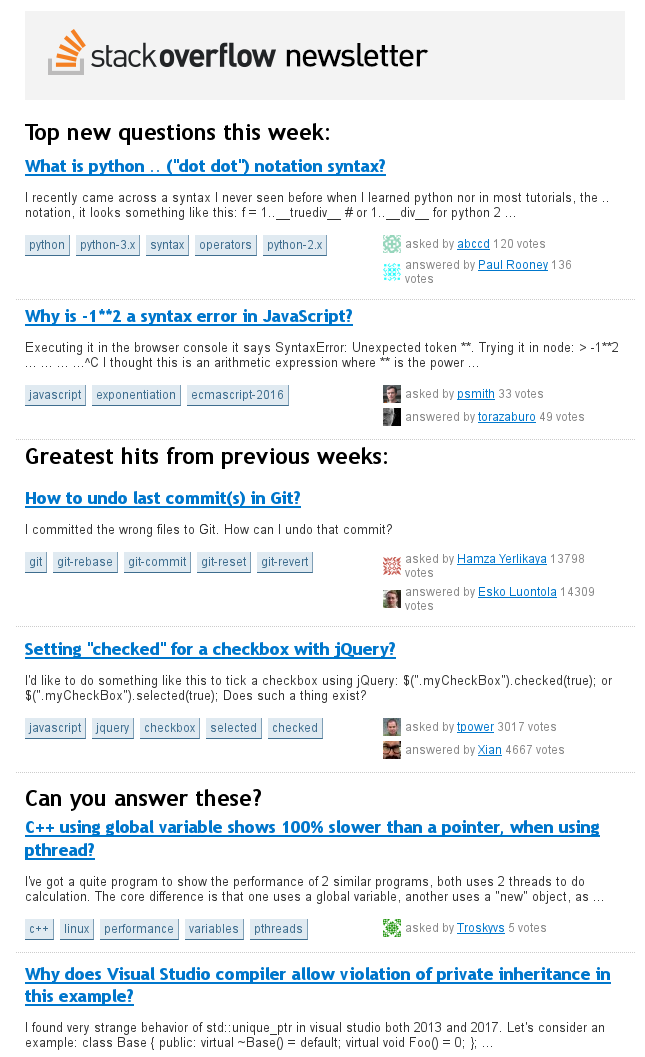
\includegraphics[scale=0.4]{so-newsletter}
\caption{Informačný bulletin komunity Stack Overflow, 25. apríl 2017.\label{fig:so-newsletter}}\end{center}
\end{figure}

\subsection{Informačný bulletin portálu Quora}

Quora\footnote{\url{https://quora.com}} je CQA systém, ktorý nie je zameraný na konkrétnu oblasť záujmu, ale obsahuje
otázky z rôznych tém. Quora ponúka svojim používateľom týždenný informačný bulletin (\emph{Quora Weekly Digest}),
ktorý obsahuje desať najzaujímavejšich otázok za posledný týždeň a zoznam ľudí, ktorých používateľ potenciálne pozná.

Zoznam najzaujímavejších otázok pozostáva z editormi manuálne vybraného obsahu a algoritmicky vybraného obsahu,
ktorý je personalizovaný pre každého používateľa zvlášť (Obr.~\ref{fig:quora-newsletter}).

\begin{figure}[H]\begin{center}
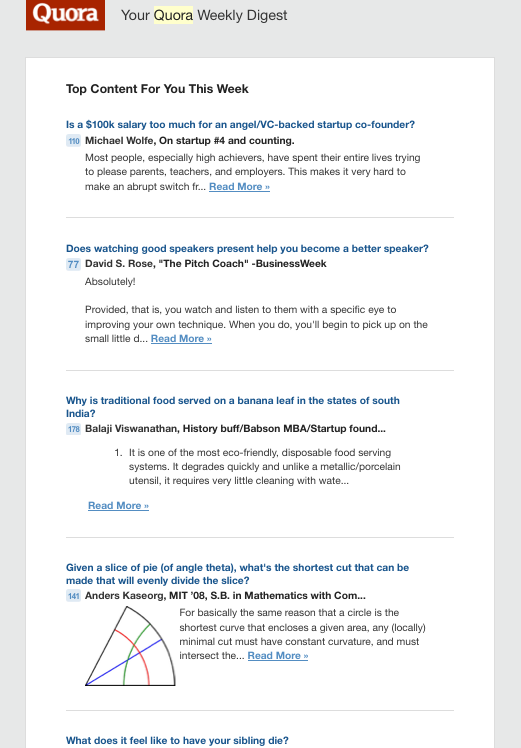
\includegraphics[scale=0.5]{quora-newsletter}
\caption{Informačný bulletin portálu Quora. Prevzaté 30.4.2017, \url{http://www.businessinsider.com/quora-emails-2012-8}
\label{fig:quora-newsletter}}\end{center}
\end{figure}

\subsection{CQA systémy bez informačných bulletinov}

Viaceré populárne CQA systémy svojim používateľom vôbec neponúkajú možnosť odoberať informačný bulletin. Medzi takéto
systémy patrí napr. portál \emph{Yahoo! Answers}\footnote{\url{https://answers.yahoo.com}}, ktorý je určený na pokladanie
otázok z akejkoľvek oblasti záujmu. Rovnako informačný newsletter neponúka ani ďalší všeobecne zameraný CQA systém --
\emph{Wiki Answers}\footnote{\url{https://answers.com}}. CQA systém zameraný na podporu výučby
\emph{Askalot}\footnote{\url{http://askalot.fiit.stuba.sk}} tiež v súčasnosti neponúka informačný newsletter,
iba možnosť notifikácie používateľa prostredníctvom e-mailu o aktivite súvisiacej s jeho obsahom v rámci systému.



%%%%%%%%%%%%%%%%%%%%%%%%%%%%%%%%%%%%%%%%%%%%%%%%%%%%%%%%%%%%%%%%%%%%%%%%%%%%%%%%%%%%%%%%%%%%%%%%%%%%%%%%%%%%%%%%%%%%%%%%


\newpage
\chapter{CQA systémy}

CQA systémy sú jednou z výrazných skupín webových portálov, ktoré sú založené na princípe používateľsky vytváraného obsahu.
Tieto systémy umožňujú používateľom položiť otázky, ktoré nie je možné zodpovedať použitím štandardných vyhľadávačov~\cite{Liu2012}
a zároveň odpovedať na otázky iných používateľov.

Napriek tomu, že väčšina CQA systémov sa spočiatku zameriava najmä na poskytnutie zmysluplnej odpovede na konkrétnu otázku,
v súčasnosti je možné v prípade niektorých CQA systémov (napr. Stack Overflow) vnímať postupnú zmenu zamerania
z jednorázových odpovedí na kolaboratívne vytváranie komplexnejších poznatkov s dlhodobou hodnotou~\cite{Anderson2012}.
Za týmto účelom CQA systémy implementujú hlasovanie a princíp reputácie ako spôsob podpory komunitného aspektu označovania
najlepších odpovedí na položené otázky.


\section{Problémy CQA systémov}

CQA systémy sa musia vysporiadavať s tými istými druhmi problémov, ako iné kategórie systémov založené na používateľmi
vytvorenom obsahu.

\subsection{Problém dlhého chvosta}
Čím viac sa zvýrazňuje trend orientácie CQA systémov viac na poskytovanie obsahu s dlhodobou hodnotou ako na samotné
poskytnutie odpovede na položenú otázku, tým viac sa prehlbuje problém \emph{dlhého chvosta} (angl. \emph{long tail}).
Ide o štandardný problém všetkých stránok zameriavajúcich sa na používateľmi vytváraný obsah, kedy je veľká väčšina
používateľov týchto stránok len pasívnymi čitateľmi (angl. \emph{lurkers}) a najväčšia časť obsahu je vytvorená len veľmi
úzkou skupinou najaktívnejších používateľov.

V prípade CQA systému Stack Overflow sa podiel aktívnych používateľov (takých, ktorí za sledovaný mesiac pridali
do systému aspoň jednu otázku alebo odpoveď) za marec 2017 pohyboval na úrovni 3\% všetkých
používateľov~\cite{Srba2016SOFail}\footnote{Výsledky za aktuálne obdobie boli získané prostredníctvom nástroja Stack
Exchange Data Explorer.}.

\subsection{Variabilita v kvalite obsahu}
Ďalším problémom CQA systémov je variabilná kvalita otázok a odpovedí v týchto systémoch. Zvyšujúcou sa popularitou CQA
systémov narastá aj podiel obsahu s nízkou kvalitou, či už vo forme veľmi jednoduchých otázok alebo nedostatočne
podrobných odpovedí, ako aj množstvo duplicitných otázok -- otázok, ktoré už boli v systéme
zodpovedané~\cite{Srba2016SOFail,Ponzanelli2014}.

Jedným z riešení tohto problému, ktorý využíva aj CQA systém Stack Overflow, je komunitné zabezpečovanie kvality obsahu
prostredníctvom moderátorov -- používateľov s oprávnením upravovať, označiť duplikát alebo vymazať obsah.


\section{Druhy CQA systémov}

CQA systémy možno kategorizovať do dvoch základných skupín podľa toho, na akú oblasť otázok sa tieto systémy zameriavajú.

\subsection{Univerzálne CQA systémy}

CQA systémy ako \emph{Yahoo! Answers}, \emph{Wiki Answers} alebo \emph{Quora} nie sú zamerané na konkrétne oblasti
a umožňujú používateľom pokladať otázky na akékoľvek témy~\cite{Chua2014}.

Tento druh CQA systémov má štandardne vyšší počet používateľov aj aktivity ako úzko špecializované CQA systémy,
no tiež tu existuje väčšia pravdepodobnosť výskytu nekvalitných, jednoduchých alebo neužitočných otázok a odpovedí,
ako aj veľký počet duplicitných otázok, ktoré už boli zodpovedané. Zároveň sú univerzálne CQA systémy zameriané viac
na samotný proces kladenia otázok a odpovedania na ne, než na vytváranie dlhodobo hodnotného obsahu.

\subsection{Úzko špecializované CQA systémy}

Opakom univerzálnych CQA systémov sú CQA systémy, ktoré sú špecializované na konkrétne oblasti záujmu.
Medzi takéto CQA systémy patria napríklad jednotlivé komunity v rámci siete Stack Exchange, ktorá zahŕňa rôzne druhy
komunít, od všeobecnejších, ako je napr. komunita venujúca sa matematike\footnote{\url{https://math.stackexchange.com}},
po veľmi úzko špecializované, akými sú napr. komunity \emph{Ask Ubuntu}\footnote{\url{https://askubuntu.com}} alebo
\emph{Raspberry Pi}\footnote{\url{https://raspberrypi.stackexchange.com}} venujúce sa konkrétnym produktom.

Tématicky zamerané CQA systémy majú väčší potenciál pre vznik dlhodobo hodnotného obsahu~\cite{Anderson2012}. V rámci
týchto systémov tiež vzniká množstvo prepojení medzi obsahom \textit{(otázky podobného charakteru, riešenie problému
v príbuznej oblasti)}, čo vedie k vzniku \emph{znalostných sietí}~(angl.~\emph{knowledge networks})~\cite{Li2016}.
S cieľom zvýšiť hodnotu jednotlivých príspevkov tiež mnohé CQA systémy zavádzajú možnosť komunitnej úpravy
otázok a odpovedí~\cite{Li2015}, čo vedie okrem zvýšenej aktivity aj k zvýšeniu vnímanej užitočnosti príspevku.



%%%%%%%%%%%%%%%%%%%%%%%%%%%%%%%%%%%%%%%%%%%%%%%%%%%%%%%%%%%%%%%%%%%%%%%%%%%%%%%%%%%%%%%%%%%%%%%%%%%%%%%%%%%%%%%%%%%%%%%%


\chapter{Odporúčanie}

\section{Odporúčacie systémy}

Odporúčacie systémy sú softvérové nástroje a techniky ktoré používateľom ponúkajú položky, ktoré by pre nich mohli
byť nejakým spôsobom zaujímavé alebo užitočné~\cite{Handbook2011}. Tieto odporúčania sú zvyčajne ponúkané za účelom
pomôcť používateľovi rozhodnúť sa, aké články by si mal prečítať, alebo aký tovar si kúpiť.

Využívanie odporúčacích systémov je tiež pre používateľov vhodným spôsobom, ako zvládať problémy informačného zahltenia
v dnešnom online svete. Ako také sa odporúčacie systémy stávajú jedným z najsilnejších a najpopulárnejších nástrojov
v online komunitách.

Odporúčacie systémy typicky vytvárajú zoznam odporúčaní jedným z dvoch spôsobov -- buď prostredníctvom \emph{kolaboratívneho
filtrovania} (angl.~\emph{Collaborative filtering}), alebo použitím \emph{filtrovania založeného na obsahu}
(angl.~\emph{Content-based filtering})~\cite{Buhmann2011}. Tieto dva prístupy môžu byť tiež kombinované
v hybridných odporúčacích systémoch.

\subsection{Kolaboratívne filtrovanie}\label{rec:collab}

Odporúčacie systémy využívajúce kolaboratívne filtrovanie fungujú prostredníctvom získavania spätnej väzby používateľa
vo forme hodnotení pre položky v danej doméne a využívajú podobnosti v hodnotení medzi viacerými používateľmi na určenie
či určitý obsah odporučiť, alebo nie~\cite{Buhmann2011}. Metódy kolaboratívneho filtrovania možno ďalej rozdeliť
na metódy založené na susednosti alebo na základe modelu.

Kolaboratívne filtrovanie na základe susednosti (angl.~\emph{Neighborhood-based Collaborative filtering})
vyberá skupinu používateľov podľa ich podobnosti k aktuálnemu používateľovi
a použitím váženej kombinácie ich hodnotení vyberá odporúčaný obsah pre tohto používateľa.
Techniky založené na modeli (angl.~\emph{Model-based Collaborative filtering}) poskytujú odporúčania prostedníctvom
oceňovania parametrov štatistických modelov pre používateľské hodnotenia.

\subsection{Filtrovanie na základe obsahu}\label{rec:content}

Odporúčanie čisto prostedníctvom kolaboratívneho filtrovania využíva iba používateľské hodnotenia. Tieto prístupy berú
všetkých používateľov a položky ako atomické jednotky a odporúčania sú vytvárané bez ohľadu na konkrétne špecifiká
individuálnych používateľov alebo položiek.

Metódy využívajúce filtrovanie na základe obsahu naopak vytvárajú
odporúčania na základe porovnávania modelov reprezentujúcich obsah s modelmi reprezentujúcimi konkrétneho používateľa.
Odporúčania v takýchto prístupoch vznikajú na základe prekryvu týchto dvoch modelov.


\section{Odporúčanie v CQA systémoch}

V kontexte CQA systémov je problematika odporúčania a odporúčacích systémov častým objektom výskumu~\cite{Srba2016}.

Jedným z hlavných cieľov CQA systémov je poskytnúť pýtajúcemu sa odpoveď na jeho otázku v čo možno najkratšom čase.
Rovnako ako v prípade iných systémov založených na používateľmi vytváranom obsahu, aj v prípade CQA systémov miera
nového obsahu -- nových otázok a odpovedí -- neustále narastá. Napriek tomu je tiež možné pozorovať stúpajúci trend
nízkej miery zodpovedanosti otázok~\cite{Srba2016SOFail}. Jedným zo spôsobov, ako je možné riešiť túto situáciu,
je práve využitie odporúčacích systémov.

V súčasnosti jedným z trendov najmä v úzko zameraných CQA systémoch ako napr. Stack Overflow, je tiež postupný prechod
od modelu jednoduchého odpovedania na položené otázky na model povzbudzujúci k vytváraniu dlhodobo hodnotného obsahu
vo forme rozsiahlych komunitne spravovaných odpovedí~\cite{Anderson2012,Li2015} podnecujúcich diskusiu.
V tomto prípade je možné využiť odporúčacie systémy ako prostriedok pre odhalenie a prezentovanie otázok a odpovedí,
ktoré by mohli používateľa zaujímať a priniesť mu úžitok~\cite{Toba2014} aj v prípade, že práve nemá rovnaký problém,
ako sa vyskytuje v danej otázke.

Výskum v oblasti odporúčania v CQA systémoch sa v súčasnosti zameriava hlavne na oblasti odporúčania, smerovania
a získavania otázok. Problémom súčasného výskumu v tejto oblasti je nejednoznačnosť a časté zamieňanie týchto výrazov,
prípadne nerozlišovanie medzi odporúčaním a smerovaním otázok~\cite{Srba2016}.

\subsection{Odporúčanie otázok}

Odporúčanie otázok (angl.~\emph{Question recommendation}) využíva tzv. \emph{pull} prístup, teda na základe (explicitnej
či implicitnej) požiadavky používateľa prezentuje zoznam odporúčaných relevantných otázok (alebo obsahu celkovo).
Tento prístup využíva štandardnejší tok medzi použitými modelmi -- začína sa modelom používateľa, na ktorý sa odporúčací
systém pokúša namapovať model relevantného obsahu.
Relevancia otázok pre používateľa môže byť identifikovaná rôznymi prístupmi -- či už na základe kolaboratívneho
filtrovania (\ref{rec:collab}) alebo filtrovania na základe obsahu (\ref{rec:content}).

Forma prezentovania odporúčaných otázok sa tiež môže líšiť. Časté je napríklad zobrazenie príbuzných otázok v detaile
konkrétnej otázky, ktorú moementálne používateľ číta. Odporúčanie otázok je však možné využiť aj ako prostriedok pre
zvýšenie záujmu a angažovanosti používateľa o CQA systém.


\subsection{Smerovanie otázok}

Na rozdiel od pomerne štandardného odporúčania otázok, v prípade smerovania otázok (angl.~\emph{Question routing})
je prístup k odporúčaniu presne opačný, a využíva tzv. \emph{push} prístup. V tomto prípade proces odporúčania začína
modelom nezodpovedanej otázky, ktorú sa snaží odporúčací systém nasmerovať k používateľovi, ktorý má najväčší potenciál
na túto otázku zodpovedať.

Výskum smerovania nezodpovedaných otázok na konkrétnych používateľov -- odpovedajúcich -- síce ukazuje, že ide o dôležitý
koncept aj z pohľadu používateľského zážitku~\cite{Li2010,Li2011}, no prináša so sebou aj problémy. Najvýraznejším z nich je zahltenie
expertov, ktorí sú hlavnými terčmi takejto formy odporúčania, nakoľko ich reputácia a expertíza ich predurčuje ako vhodných
kandidátov na zodpovedanie veľkého množstva otázok~\cite{Pal2015}.

Pomerne novým prístupom k smerovaniu otázok je namiesto zamerania na konkrétnych používateľov smerovanie otázok na väčšie
komunity používateľov~\cite{Liu2014}. Hlavnou ideou takéhoto smerovania je fakt, že kolektívne poznatky komunity sú vždy väčšie, ako
poznatky konkrétneho používateľa, aj experta~\cite{Pal2013}. Navyše takéto smerovanie zvyšuje pravdepodobnosť rýchlejšieho zodpovedania
otázky, ako aj zabraňuje zahlteniu expertov. Hlavným problémom smerovania na komunity je vytváranie kolektívneho modelu
reprezentujúceho komunitu, kedy je potrebné brať do úvahy okrem iného fakt, že iba malá časť komunity sú \emph{tvorcovia
poznatkov} a nie len ich konzumenti~\cite{Pal2015}.


\subsection{Získavanie otázok}

Tento pojem (angl.~\emph{Question retrieval}) v kontexte CQA systémov hovorí o procese vyberania podobných otázok pre
rôzne formy dopytov~\cite{Zhang2014} na základe syntaktickej podobnosti otázok.
Tento proces je možné využiť na hľadanie odpovedí alebo poznatkov vo veľkých množstvách už zodpovedaných otázok.


\subsection{Problém studeného štartu}\label{cold-start}

Častým problémom odporúčania je problém studeného štartu (angl.~\emph{Cold start}), kedy je na dosiahnutie primeranej
miery presnosti odporúčania potrebné veľké množstvo informácií, ktoré ale napr. v prípade nových alebo menej aktívnych
používateľov nemusia byť k dispozícii.

Tento problém sa vyskytuje najmä v prípade systémov, ktoré obsah odporúčajú na základe
podobnosti používateľov medzi sebou. Keďže je často na začiatok potrebné veľké množstvo informácií o daných používateľoch,
nie je možné jednoducho odporúčať vhodný obsah pre používateľov, ktorí sú menej aktívni, alebo sú noví.
V menšej miere týmto problémom trpia systémy, ktoré namiesto podobnosti používateľov využívajú pre zostavovanie odporúčaní
podobnosť samotného obsahu na základe rôznych atribútov.

\subsection{Segmentácia používateľov}

Ďalším z problémov v oblasti personalizovaného odporúčania, veľmi výrazným aj v prípade informačných bulletinov,
je rozdelenie používateľov zaujímajúcich sa o informačný bulletin do skupín podľa účelu, za ktorým chcú informačný bulletin dostávať.
V prípade úzko zameraných CQA systémov, ako je napr. Stack Overflow, je možné používateľov rozdeliť do dvoch základných
skupín -- producentov a konzumentov.

Producenti sú používatelia, ktorí primárne odpovedajú na otázky. Takýto používatelia
tvoria dôležitú časť komunity~\cite{Anderson2012}. Motiváciou pre odoberanie informačného bulletinu pre takýchto používateľov
je hlavne potenciál identifikovať otázky, ktoré ešte neboli dostatočne alebo správne zodpovedané, prípadne záujem
o diskusiu o zaujímavých a netriviálnych otázkach. Konzumenti sú zase používatelia, ktorí sú spravidla v rámci komunity
používateľov menej aktívni a ich motiváciou je zbierať vedomosti~\cite{Anderson2012}. Pre týchto používateľov je potrebné
identifikovať vysoko kvalitné odpovede na otázky~\cite{Toba2014}.

Jednotlivé skupiny používateľov tak prirodzene očakávajú nie len iný druh otázok, ale aj celé odlišné súčasti informačných bulletinov.


\subsection{Problém filtračnej bubliny}\label{rec:filterbubble}

Ďalším problémom, ktorému sa však v oblasti odporúčania obsahu CQA systémov venuje menej pozornosti~\cite{Srba2016},
je rôznorodosť odporúčaného obsahu. Hrozí tak výskyt problému tzv. filtračnej bubliny (angl.~\emph{Filter bubble}).

Ak totiž systém používateľovi odporúča obsah len z oblastí používateľovho záujmu, dochádza k problému, kedy je používateľ
do značnej miery uzatvorený v rámci jednej oblasti a nemá tak možnosť získavať zaujímavé poznatky z iných oblastí.
Používateľ sa tak síce môže stať odborníkom na danú oblasť, no jeho povedomie o širšom kontexte celej problematiky
je veľmi obmedzené.

Riešením tohto problému je identifikácia oblastí, ktoré nie sú priamo oblasťami záujmu používateľa, no sú k týmto
oblastiam v určitých aspektoch príbuzné. Používateľ má tak možnosť rozšíriť svoj okruh záujmu a vedomosti o širšom
kontexte problémovej domény.


%%%%%%%%%%%%%%%%%%%%%%%%%%%%%%%%%%%%%%%%%%%%%%%%%%%%%%%%%%%%%%%%%%%%%%%%%%%%%%%%%%%%%%%%%%%%%%%%%%%%%%%%%%%%%%%%%%%%%%%%


\chapter{Diverzita a aktuálnosť odporúčania}

Diverzitu možno všeobecne definovať ako opak podobnosti. V niektorých prípadoch však nemusí byť odporúčanie podobných
položiek tým najlepším riešením pre používateľa~\cite{Handbook2011}. Dôvodom je práve náchylnosť takéhoto odporúčania na
vyvolanie problému filtračnej bubliny (viď kapitola \ref{rec:filterbubble}).

Okrem diverzifikácie odporúčaného obsahu má na celkovú úspešnosť vytvárania personalizovaných odporúčaní veľký vplyv aj
aktuálnosť (angl.~\emph{freshness}, príp.~\emph{novelty}) odporúčaného obsahu~\cite{Liu2015}.

\section{Diverzita v odporúčacích systémoch}

Tématická diverzifikácia je metóda napomáhajúca vyváženosti a diverzite personalizovaného odporúčania s cieľom
lepšie reflektovať kompletné spektrum používateľových záujmov. Napriek tomu, že môže mať negatívny vplyv na priemernú
správnosť odporúčaní, dosahuje táto metdóda zvýšenú úroveň používateľskej spokojnosti~\cite{Zhang2009}.

Ziegler a kol.~\cite{Ziegler2005} študovali diverzifikáciu v oblasti odporúčaní a navrhli prístup, ktorý vytvára
zoznamy odporúčaní lepšie uspokojujúce používateľove záujmy prostredníctvom selekcie takých zoznamov, ktoré majú nízku
vnútornú podobnosť. Autori v experimente demonštrovali, že reálny používatelia preferujú diverznejšie výsledky.

Tradičný spôsob zavedenia diverzity do odporúčania je diverzifikácia na základe atribútov odporúčaného obsahu, teda
zoskupenie výsledkov do skupín zdieľajúcich viaceré atribúty (ako napr. žáner hudby) a následný výber iba limitovaného
množstva výsledkov z každej zo skupín. Autori v~\cite{Yu2009} prezentujú \emph{diverzifikáciu na základe dôvodu}.
Táto metóda využíva pre diverzifikáciu výsledkov dôvod, prečo bola konkrétna položka odporučená
(napr. \textit{tento album bol odporučený, pretože ste počúvali inú skladbu tohto autora}). Autori experimentálne ukázali,
že takáto forma diverzifikácie je prinajmenšom rovnako účinná, ako diverzifikácia na základe atribútov položiek.

Inú perspektívu volí metóda diverzity na báze proporcionality. Zoznam odporúčaní je možné považovať za najlepšie diverzifikovaný
vzhľadom na relevanciu odporúčaní v takom prípade, keď počet výsledkov z určitej témy je úmerný popularite danej témy.
Dang a kol. vo svojej práci~\cite{Dang2012} ponúkajú koncept optimalizácie proporčnosti pre diverzifikáciu výsledkov
vyhľadávania.

Napriek tomu, že sa táto práca nezaoberá priamo diverzitou v odporúčacích systémov, sú paralely s touto
oblasťou výrazné. Motiváciou pre tákyto spôsob diverzifikácie je metóda obsadzovania kresiel v parlamente. Ich metóda
postupne pre každú pozíciu v zozname výsledkov určuje tému, ktorá najlepšie zachováva celkovú proporčnosť. Následne
na túto pozíciu z danej témy vyberie najlepší dokument.


\section{Aktuálnosť v odporúčacích systémoch}

Aktuálnosť v kontexte odporúčacích systémov môže predstavovať dva rôzne aspekty. Jedným z nich je \emph{novosť}
(angl.~\emph{novelty}), teda pomerne priamočiara vlastnosť určujúca, či odporúčaný obsah už bol používateľovi prezentovaný,
alebo nie. Jednoduchým spôsobom, ako zabezpečiť, aby používateľovi neboli stále dookola odporúčané tie isté položky,
akokoľvek relevantné by pre neho mohli byť, je odfiltrovanie položiek, ktoré už používateľovi boli odporúčané v minulosti,
a s ktorými už interagoval~\cite{Handbook2011}.

Druhým aspektom aktuálnosti je \emph{čerstvosť} (angl.~\emph{freshness}). V tomto prípade ide o časovú aktuálnosť odporúčaného
obsahu. Naivný prístup k aktuálnosti je odporúčanie iba obsahu z určitého obmedzeného časového úseku z blízkej minulosti,
no takýto prístup nemusí vždy dosahovať najlepšie výsledky používateľskej spokojnosti~\cite{Szpektor2013}.

Pri odporúčaní, ktoré berie do úvahy aktuálnosť odporúčaného obsahu je dôležitým aspektom detekcia časovo citlivej témy.
Takýto systém by mal brať presadzovať aktuálny obsah iba v prípade, kedy je to vhodné. Na druhej strane, ak je v prípade
aktívne sa vyvýjajúcej témy odporúčaný neaktuálny obsah, môže to výrazne degradovať úspešnosť odporúčania~\cite{Dong2010}.
Ďalším faktorom pri posudzovaní aktuálnosti v odporúčaní je časová škála aktuálnosti pre danú tému.
V prípade niektorých tém alebo oblastí je možné považovať za aktuálne položky z posledného roka, no v iných prípadoch
môžu byť aj niekoľko týždňov staré položky považované za vysoko neaktuálne.

Ďalším problémom vzhľadom na aktuálnosť v odporúčaní je tiež fakt, že pre novo vzniknutý obsah môže byť problémovejšie
zostaviť model, ktorý by ho reprezentoval, nakoľko môže byť o tomto obsahu známych zatiaľ iba málo informácií~\cite{Dong2010TW}.
Tento problém studeného štartu sa môže prejavovať rovnako v prípade modelovania obsahu, ako je tomu napríklad v prípade
vytvárania modelov reprezentujúcich nových používateľov.

Riešením v takomto prípade môže byť napríklad vytváranie modelu
obsahu na základe čŕt, ktoré nie sú ovplyvnené časom (napr. nadpis, text alebo autor obsahu, na rozdiel od počtu hlasov
alebo dátumu uverejnenia), alebo tiež upravenie hodnôt týchto čŕt vzhľadom na relatívnu aktuálnosť obsahu.


\section{Diverzita a aktuálnosť v kontexte CQA systémov}

Kým diverzita a aktuálnosť sú v oblasti odporúčania a celkovo vo vyhľadávaní informácií pomerne často analyzovanými aspektmi,
v kontexte CQA systémov sa týmto hľadiskám doteraz venovala iba okrajová pozornosť~\cite{Srba2016}.

Liu a kol. vo svojej práci~\cite{Liu2015} skúmajú aspekt aktuálnosti odporúčania v CQA systémoch prostredníctvom
relatívne neštandardného návrhu CQA systému určeného pre odpovedanie v reálnom čase na \emph{hyper-lokálne} a časovo senzitívne
otázky. Za týmto účelom využívajú prístupy predchádzajúcich prác a kombinujú aspekty relevancie, lokality a aktuálnosti
v \emph{real-time} CQA systéme.


Komplexnejší pohľad na aktuálnosť a diverzitu priamo v kontexte štandardných CQA systémov ponúka Szpektor a kol~\cite{Szpektor2013}.
Autori experimentovali so zavedením diverzity a aktuálnosti do procesu vytvárania odporúčaní pre používateľov CQA
systému Yahoo! Answers, pričom sa na rozdiel od väčšiny prác v tejto oblasti nezameriavali len na skupinu expertných používateľov.

Pre odporúčanie využili profil otázok založený na kombinácii LDA, lexikálneho a kategorického modelu a profil používateľa
odvodený od profilu otázok, s ktorými interagoval. Párovanie otázok a používateľov bolo vykonané prostredníctvom jednoduchého
skalárneho súčinu vektorov reprezentujúcich profily používateľov a otázok.

Samotná diverzifikácia odporúčaní bola vykonávaná prostredníctvom tématického výberu vzoriek (angl.~\emph{thematic sampling}),
kedy je vygenerovaných viacero samostatných zoznamov odporúčaných otázok z viacerých tém, ktoré sú následne zmiešané dokopy
proporcionálne k pravdepodobnostnému skóre jednotlivých tématických zoznamov.

Prínos aktuálnosti do odporúčania v CQA systémoch bol skúmaný na základe odporúčania iba aktuálneho obsahu -- konkrétne
iba nezodpovedaných otázok za posledné štyri hodiny.

Dopad diverzifkácie a aktuálnosti na úspešnosť odporúčania bol testovaný v rámci online experimentu. Používatelia boli náhodne
rozdelení do štyroch segmentov:

\begin{my_enumerate}
  \item{\textbf{Kontrolná vzorka} -- Týmto používateľom neboli ponúknuté žiadne odporúčania.}
  \item{\textbf{Odporúčanie na základe relevancie} -- Používateľom boli ponúknuté odporúčania iba na základe relevancie
        daných otázok, bez ohľadu na aktuálnosť alebo diverzitu.}
  \item{\textbf{Odporúčanie s ohľadom na aktuálnosť} -- Používateľom boli odporúčané relevantné otázky, pričom 50\% z nich
        pochádzalo z posledných štyroch hodín a 20\% bolo vybraných prostredníctvom tématického výberu vzoriek.}
  \item{\textbf{Diverzifikované odporúčanie} -- Používateľom boli odporúčané relevantné otázky, pričom 50\% z nich
        bolo vybraných na základe tématického výberu vzoriek ako prostriedku diverzifikácie, a 20\% pochádzalo z posledných
        štyroch hodín.}
\end{my_enumerate}

Výsledky online experimentu potvrdili intuitívnu myšilienku, že iba samotná relevancia nie je dostatočná na úspešne
odporúčanie otázok v CQA systéme. Práve naopak, vo vykonanom experimente dokonca samotné odporúčanie len na základe
relevancie dosiahlo nižšie hodnoty zodpovedania otázok, ako kontrolná vzorka bez akýchkoľvek odporúčaní.

Presadzovanie aktuálnych otázok dosiahlo zvýšenie miery zodpovedania otázok o 4\%, avšak najlepšie výsledky boli dosiahnuté
prostredníctvom diverzifikácie odporúčaní aj za cenu zníženia aktuálnosti, pričom miera zodpovedania sa zvýšila o 17\%.

\vspace*{1.5cm}

Na základe tejto analýzy môžeme usúdiť, že napriek tomu, že problematika diverzifikácie a aktuálnosti odporúčania v kontexte
CQA systémov v súčasnosti stále ostáva do veľkej miery nepreskúmaná, je očividné, že uvažovanie týchto aspektov v tomto
kontexte má veľký vplyv na úspešnosť odporúčania, pričom informačné bulletiny sa javia ako prirodzená, požadovaná,
no napriek tomu málo využívaná forma prinášania odporúčaného a potenciálne zaujímavého obsahu použivateľom.


%%
%% design
%%
%!TEX root = main.tex
\newpage
\chapter{Návrh riešenia personalizovaného informačného bulletinu v CQA systéme}

Cieľom našej práce je navrhnúť a overiť metódu zostavovania personalizovaných informačných bulletinov v CQA systémoch
so zameraním na podporu diverzity a aktuálnosti odporúčaného obsahu.

\section{Dáta v doméne CQA systémov}

Experimenty s personalizáciou informačných bulletinov budeme realizovať na platforme Stack Exchange, ktorá patrí medzi
najpopulárnejšie CQA systémy súčasnosti a tvorí ju viac ako 160 samostatných komunít zameraných na rôzne oblasti.

Experimenty plánujeme vykonávať nad dátami z komunity \textit{Software Engineering}\footnote{\url{http://softwareengineering.stackexchange.com}},
nakoľko je táto komunita zameraná na doménu, v ktorej máme hlbšie vedomosti a teda vieme lepšie posúdiť správnosť
odporúčania v tejto doméne. Navrhnuté riešenie však nebude špecifické pre túto komunitu, našim cieľom je naopak vytvoriť
metódu, ktorú bude možné nasadiť v rámci celej platformy Stack Exchange, rovnako ako na iných CQA systémoch s podobnou
štruktúrou.

Platforma Stack Exchange pravidelne zverejňuje kompletné archívne dáta zo všetkých komunít vo forme XML výstupov reflektujúcich
entity systému. Tieto dáta plánujeme využiť v prvotnej fáze experimentov na vytvorenie základných modelov.
Pre následné zdokonaľovanie modelov, ako aj zabezpečenie aktuálnosti použitých dát budeme využívať verejné API poskytované
platformou Stack Exchange.

\subsection{Charakteristika dát}

\subsubsection{Archívne dáta}
Dáta v dátovom archíve platformy Stack Exchange\footnote{\url{http://archive.org/details/stackexchange}} sú pravidelne
aktualizované a obsahujú kompletné používateľmi vytvorené anonymizované dáta zo všetkých komunít platformy.
Všetky tieto dáta sú verejne dostupné pod licenciou \emph{Creative Commons Attribution-ShareAlike 3.0 Unported}.

Štruktúra dát v archívoch je nasledovná:

\begin{my_itemize}
  \item{\textit{Badges.xml} -- Obsahuje ID používateľov, názvy odznakov a čas, kedy používateľ daný odznak získal.}
  \item{\textit{Comments.xml} -- Obsahuje všetky komentáre spolu s informáciou o ich autoroch a príspevkoch, ku ktorým sa viažu.}
  \item{\textit{Posts.xml} -- Obsahuje informácie o všetkých príspevkoch (otázkach a odpovediach) a k nim prislúchajúce značky, ako aj aktuálne znenie príspevku}
  \item{\textit{PostHistory.xml} -- Obsahuje históriu zmien jednotlivých príspevkov, ako napr. zmenu názvu, štítkov, označenie otázky za zodpovedanú a pod.}
  \item{\textit{PostLinks.xml} -- Obsahuje informácie o prepojeniach medzi príspevkami, konkrétne o duplikátoch a príbuzných príspevkoch.}
  \item{\textit{Users.xml} -- Obsahuje verejné údajé všetkých používateľov, ako sú meno, reputácia, webová stránka, počet hlasov a iné.}
  \item{\textit{Votes.xml} -- Obsahuje anonymizované informácie o hlasoch príspevkov.}
\end{my_itemize}


\subsubsection{Stack Exchange API}

API platformy Stack Exchange\footnote{\url{http://api.stackexchange.com}} poskytuje prístup ku všetkým verejným dátam
platformy v reálnom čase. API podporuje dvojúrovňový prístup k dátam.

\textbf{Obmedzenia požiadaviek}\\
Menšie aplikácie môžu využiť základnú úroveň, ktorá na používanie nevyžaduje registráciu a autentifikáciu,
no jej prístup podlieha obmedzovaniu v miere prístupu a môže z jednej IP adresy denne vykonať iba 10 000 požiadaviek na API.

V prípade, že aplikácia využívajúca API vykoná autentifikáciu používateľa, je limit 10 000 požiadaviek denne špecifický
pre každého používateľa zvlášť.

Bez ohľadu na úroveň prístupu je tiež uplatňované limitovanie na 30 požiadaviek za sekundu z jednej IP adresy, ako aj
dynamické limitovanie, ktoré spočíva v tom, že každá odpoveď API môže obsahovať parameter indikujúci počet sekúnd, koľko
má aplikácia počkať pred vykonaním ďalšej požiadavky. Tento limit musí dodržiavať každá aplikácia.

\textbf{Vlastné filtre}\\
Stack Exchange API umožňuje flexibilne špecifikovať jednotlivé atribúty, ktoré majú byť vrátené v odpovedi na požiadavku.
Táto podpora je implementovaná prostredníctvom filtrov, ktoré môže aplikácia využívajúca API vytvoriť. Každý filter môže
obsahovať (1) zoznam atribútov, ktoré majú byť prítomné, (2) atribúty, ktoré nemajú byť súčasťou odpovede a (3) základný
filter, od ktorého je daný filter odvodený.\\
Použitie filtrov umožňuje aplikáciám pokladať efektívnejšie požiadavky, ktoré vrátia iba všetky aplikáciou požadované
atribúty a nič navyše.

\textbf{Autentifikácia}\\
Autentifikácia používateľov pri použití API je implementovaná prostredníctvom otvoreného štandardu
OAuth 2.0\footnote{\url{http://oauth.net}}. Pre využívanie autentifikovaných požiadaviek v API je nutné zaregistrovať
aplikáciu v centrálnom zozname všetkých aplikácií využívajúcich API platformy Stack Exchange --
\textit{Stack Apps}\footnote{\url{http://stackapps.com}}.

\subsubsection{Rozsah dát}

Komunita \textit{Software Engineering}, ktorú budeme využívať v experimentoch pri návrhu riešenia má nasledovný rozsah:

\begin{my_itemize}
    \item{Otázky - cca 45 tisíc}
    \item{Odpovede - cca 138 tisíc}
    \item{Používatelia - cca 221 tisíc}
    \item{Pridelené odznaky - cca 405 tisíc}
    \item{Komentáre - cca 397 tisíc}
    \item{Značky - cca 1.6 tisíc}
    \item{Miera zodpovedanosti otázok - cca 94\%}
\end{my_itemize}


\section{Návrh metódy personalizovaného odporúčania}

\textbf{Hypotéza}\\
\textit{Použitím personalizovaného odporúčania otázok v informačnom bulletine CQA systému zvýšime relevanciu obsahu informačného
bulletinu, čo sa prejaví zvýšenou aktivitou používateľov CQA systému.}

Pri vytváraní personalizovaného informačného bulletinu sa budeme zameriavať na odporúčanie relevantných otázok jednotlivým
používateľom CQA systému prostredníctvom metódy filtrovania na základe obsahu (kapitola \ref{rec:content}). Za týmto účelom
je potrebné zostaviť modely reprezentujúce otázky a používateľov systému.

\subsection{Model otázok}

Model otázok bude zložený z troch nezávislých modelov, ktoré sa na otázky pozerajú z rôznych perspektív.

\begin{my_enumerate}
\item{\textbf{Kategorický model otázok}\\
Tento model reprezentuje otázku na najvyššej úrovni ako prislúchajúcu do určitých kategórií. Kategórie otázok sú v rámci
platformy Stack Exchange reprezentované ako značky (angl.~\emph{tags}). Každá otázka môže obsahovať viacero značiek, pričom
platforma identifikuje aj synonymické značky, ktoré možno chápať ako bližšie určenie kategórie.}

\item{\textbf{LDA tématický model}\\
Tento model využíva metódu latentnej Dirichletovej alokácie (angl.~\emph{Latent Dirichlet Allocation})~\cite{blei2003latent}
na určenie témy, ktorej sa daná otázka venuje. LDA vektor je vypočítaný z nadpisu a samotného textu otázky.}

\item{\textbf{Komunitný model}\\
\textit{Komunitný model} je naše pomenovanie pre model reprezentujúci komunitný faktor danej otázky. Predstavuje ho vektor
zložený z viacerých čŕt, ako napr. počet hlasov, počet odpovedí, atď. Presný zoznam použitých čŕt obsahuje
kapitola~\ref{features}. Tento model predstavuje prínos a hodnotu otázky pre komunitu.}
\end{my_enumerate}


\subsection{Model používateľov}

Model používateľa bude vytvorený prostredníctvom agregácie modelov otázok, s ktorými používateľ v minulosti interagoval
-- či už ich pokladal, odpovedal na ne, alebo za otázku hlasoval, okomentoval ju alebo ju označil za obľúbenú.

Druh interakcie používateľa s otázkou bude mať dopad na faktor, s akým bude daná interakcia agregovaná -- menšie interakcie
(hlasovanie, komentár) budú brané do úvahy menej ako napr. odpovedanie alebo samotné položenie otázky.

S cieľom reflektovať časom sa meniace preferencie používateľa bude tiež aplikovaný faktor zmeny (angl.~\emph{decaying factor}).


\subsection{Výber odporúčaného obsahu}\label{rec-retrieval}

Pre účely zostavovania zoznamu odporúčaných otázok použijeme prístup analogický štandardným nástrojom pre vyhľadávanie
informácií (angl.~\emph{Information Retrieval Engines}). V našom prípade budú dokumentmi samotné otázky a dopytom bude
model používateľa. Pre ohodnocovanie podobnosti modelov bude použitý skalárny súčin vektorov reprezentujúcich
modely otázky a používateľa.


\subsection{Riešenie problému studeného štartu}

Pre eliminovanie problému studeného štartu (kapitola~\ref{cold-start}) z pohľadu prvotného odporúčania otázok využijeme
offline natrénovanie našich metód na archívnych dátach platformy Stack Exchange.

V prípade nových používateľov, ktorí v systéme nemajú žiadnu, alebo iba nedostatočnú aktivitu, budeme zo začiatku vytvárať
iba generický informačný bulletin podobný tomu, ktorý je používateľom k dispozícii aj v súčasnosti (kapitola~\ref{so-newsletter}).


\section{Návrh metódy diverzifikácie odporúčaní}

\textbf{Hypotéza}\\
\textit{Výberom odporúčaných otázok zo širšieho okruhu záujmu používateľa a zohľadnením ich aktuálnosti predídeme výskytu problému
filtračnej bubliny, čím dosiahneme vyššiu mieru záujmu používateľa a jeho aktivity.}

Pre účely diverzifikácie odporúčaných otázok budeme porovnávať výsledky dvoch rôznych metód diverzifikácie.

\subsection{Tématické vzorkovanie}
Metódu diverzifikácie prostredníctvom tématického vzorkovania sme navrhli nasledovne:

\begin{my_enumerate}
\item{
  Pre každého používateľa vyberieme náhodne N rôznych tém, ktoré sú pre neho relevantné. Tieto témy sa vyberú zo zoznamu
  kategórií a LDA tém z modelu používateľa.
}
\item{
  Prostredníctvom vyššie opísaného mechanizmu (kapitola~\ref{rec-retrieval}) vyberieme pre každú takúto tému zoznam
  odporúčaní.
}
\item{
  Následne sa budú z jednotlivých zoznamov vyberať samotné položky do výsledného zoznamu odporúčaní. Pravdepodobnosť výberu
  otázky z konkrétneho zoznamu bude proporčná k relevancii tejto témy pre daného používateľa.
}
\item{
  Pravidlá pre výber konkrétnych otázok z jednotlivých zoznamov zatiaľ nešpecifikujeme. Pre účely zvýšenia diverzity však
  nepredpokladáme jednoduchý výber podľa poradia v rámci zoznamu, ale aplikovanie inej distribúcie, prípadne náhodný výber.
}
\end{my_enumerate}

Proces tématického vzorkovania ilustruje Obrázok~\ref{fig:tematic-sampling}.


\subsection{Proporčná diverzifikácia}
Táto metóda diverzifikácie je vo svojej podstate jednoduchšia a priamočiarejšia ako tématické vzorkovanie. Spočíva
vo výbere N najrelevantnejších tém, pričom témy sú definované rovnako, ako v prípade tématického vzorkovania.
Samotné otázky zo zoznamov jednotlivých tém sú vyberané od vrchu podľa ich ohodnotenia.


\section{Výber čŕt pre použitie v metódach}\label{features}

\begin{my_itemize}
  \item Črty otázok
  \begin{my_itemize}
    \item Nadpis otázky
    \item Text otázky
    \item Značky priradené k otázke
    \item Dátum poslednej zmeny
    \item Počet hlasov - skóre
    \item Počet zobrazení
    \item Počet označení za obľúbenú
    \item Má/nemá akceptovanú odpoveď
    \item Počet odpovedí
    \item Súhrnný počet komentárov (počet komentárov na otázke aj odpovediach)
    \item Počet zmien v otázke
    \item Reputácia autora otázky
    \item Reputácia autora akceptovanej odpovede
  \end{my_itemize}
  \item Črty používateľov
  \begin{my_itemize}
    \item Reputácia používateľa
    \item Počet kladných hlasov
    \item Počet záporných hlasov
    \item Počet položených otázok
    \item Počet komentárov
    \item Počet poskytnutých odpovedí
    \item Dátum registrácie
    \item Dátum poslednej aktivity
  \end{my_itemize}
\end{my_itemize}

\section{Metriky hodnotenia výsledkov}

Pre overovanie výsledkov experimentov budeme používať tieto metriky:

\textbf{Precision@N}\\
Presnosť (angl.~\emph{Precision}), alebo tiež \textit{pozitívna predikčná hodnota} je metrika reprezentujúca pomer relevantných
dokumentov z celkového zoznamu. Štandardne sa presnosť počíta ako pomer z celého zoznamu dokumentov, no v oblasti
odporúčania a vyhľadávania informácií je často vhodnejšou odvodená metrika \textit{Precision@N}, ktorá určuje, aká časť
z prvých N dokumentov v zozname je relevantná.

\textbf{nDCG}\\
\textit{Normalized Discounted Cumulative Gain} je metrika kvality ohodnocovania často používaná na meranie efektívnosti
odporúčania. DCG meria užitočnosť dokumentov na základe ich pozície vo výslednom zozname. Užitočnosť dokumentov sa akumuluje
od konca zoznamu, pričom najvyššiu užitočnosť majú dokumenty na začiatku zoznamu~\cite{Jrvelin2002}.

\textbf{CTR}\\
Miera preklikov (angl.~\emph{Click-through Rate}) je metrika často využívaná v spojitosti s informačnými bulletinmi.
Táto metrika vyjadruje počet úspešných kliknutí na odkaz v informačnom bulletine.

Okrem CTR plánujeme v súvislosti s interakciou používateľa s informačným bulletinom merať aj počet impresií,
teda zobrazení informačného bulletinu, ako aj počet konverzií, teda podiel prípadov, kedy kliknutie na niektorú z otázok
v informačnom bulletine viedlo k aktivite používateľa na tejto otázke -- či už hlasovanie, odpovedanie alebo pridanie komentáru.


\section{Návrh overenia metód}

Nami navrhnuté metódy personalizovaného odporúčania a diverzifikácie odporúčaného obsahu budeme overovať prostredníctvom
online nekontrolovaného experimentu na používateľoch z komunity \textit{Software Engineering} platformy Stack Exchange.

Tento online experiment bude mať formu pravidelne rozposielaného informačného bulletinu, na ktorého odoberanie sa budú
môcť prihlásiť všetci používatelia z tejto komunity.

Účinnosť zvolených metód diverzifikácie odporúčaní budeme vyhodnocovať prostredníctvom A/B testovania, pričom používateľov
rozdelíme na tri skupiny:
\begin{my_enumerate}
    \item{Kontrolná skupina -- odporúčania nebudú diverzifikované}
    \item{Skupina A -- využitie metódy tématického vzorkovania}
    \item{Skupina B -- využitie metódy proporčnej diverzifikácie}
\end{my_enumerate}

Dôležitým predpokladom pre úspešnosť online experimentu bude získať dostatočnú reprezentatívnu vzorku používateľov
ochotných byť súčasťou experimentu. V prípade, že by sa nám nepodarilo osloviť dostatočný počet používateľov, plánujeme
vykonať kontrolovaný offline experiment na vzorke archívnych dát.



%%
%% implementation
%%
%!TEX root = main.tex
\newpage
\chapter{StackLetter -- personalizovaný informačný bulletin pre Stack Exchange}

\textit{StackLetter} je systém pre vytváranie a rozosielanie personalizovaných informačných bulletinov vrámci platformy
Stack Exchange. Tento systém sme vyvinuli spoločne s kolegom Bc. Matúšom Salátom~\cite{Salat2018}. Celý systém sa skladá
z viacerých spolupracujúcich modulov, ktoré však boli vyvíjané samostatne a sú od seba navzájom nezávislé. Rozdelenie
systému na nezávislé moduly umožňuje rýchlejší vývoj, ako aj možnosť jednoduchého rozširovania systému v budúcnosti.
Architektonický prehľad celého systému znázorňuje obrázok~\ref{fig:architecutre-overview}. Ďalej v tejto práci popisujem
len mnou navrhnuté moduly.

\begin{figure}[H]\begin{center}
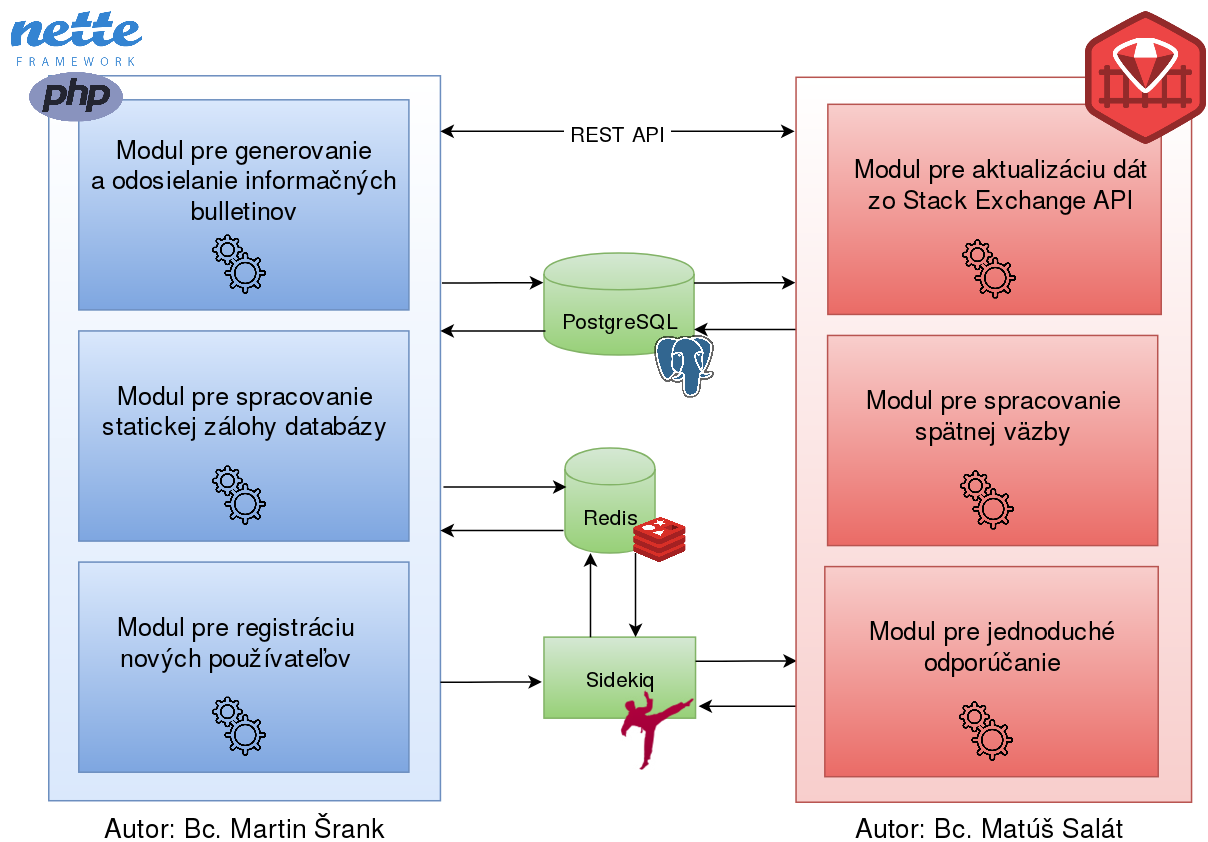
\includegraphics[scale=0.37]{architecture-overview}
\caption{Architektonický prehľad systému StackLetter. \label{fig:architecutre-overview}}\end{center}
\end{figure}

\section{Prehľad modulov}

\textbf{Modul pre registráciu nových používateľov}\\
Tento modul predstavuje používateľmi viditeľnú časť systému. Prostredníctvom webovej stránky systému
-- \url{www.stackletter.com} -- sa používatelia môžu prihlásiť k odoberaniu informačného bulletinu pre niektoré
z ponúkaných komunít platformy Stack Exchange, ako aj spravovať svoje nastavenia týkajúce sa odosielania informačných
bulletinov.\\
Používatelia sa prihlasujú prostredníctvom svojho Stack Exchange konta využitím protokolu OAuth.

\begin{figure}[H]\begin{center}
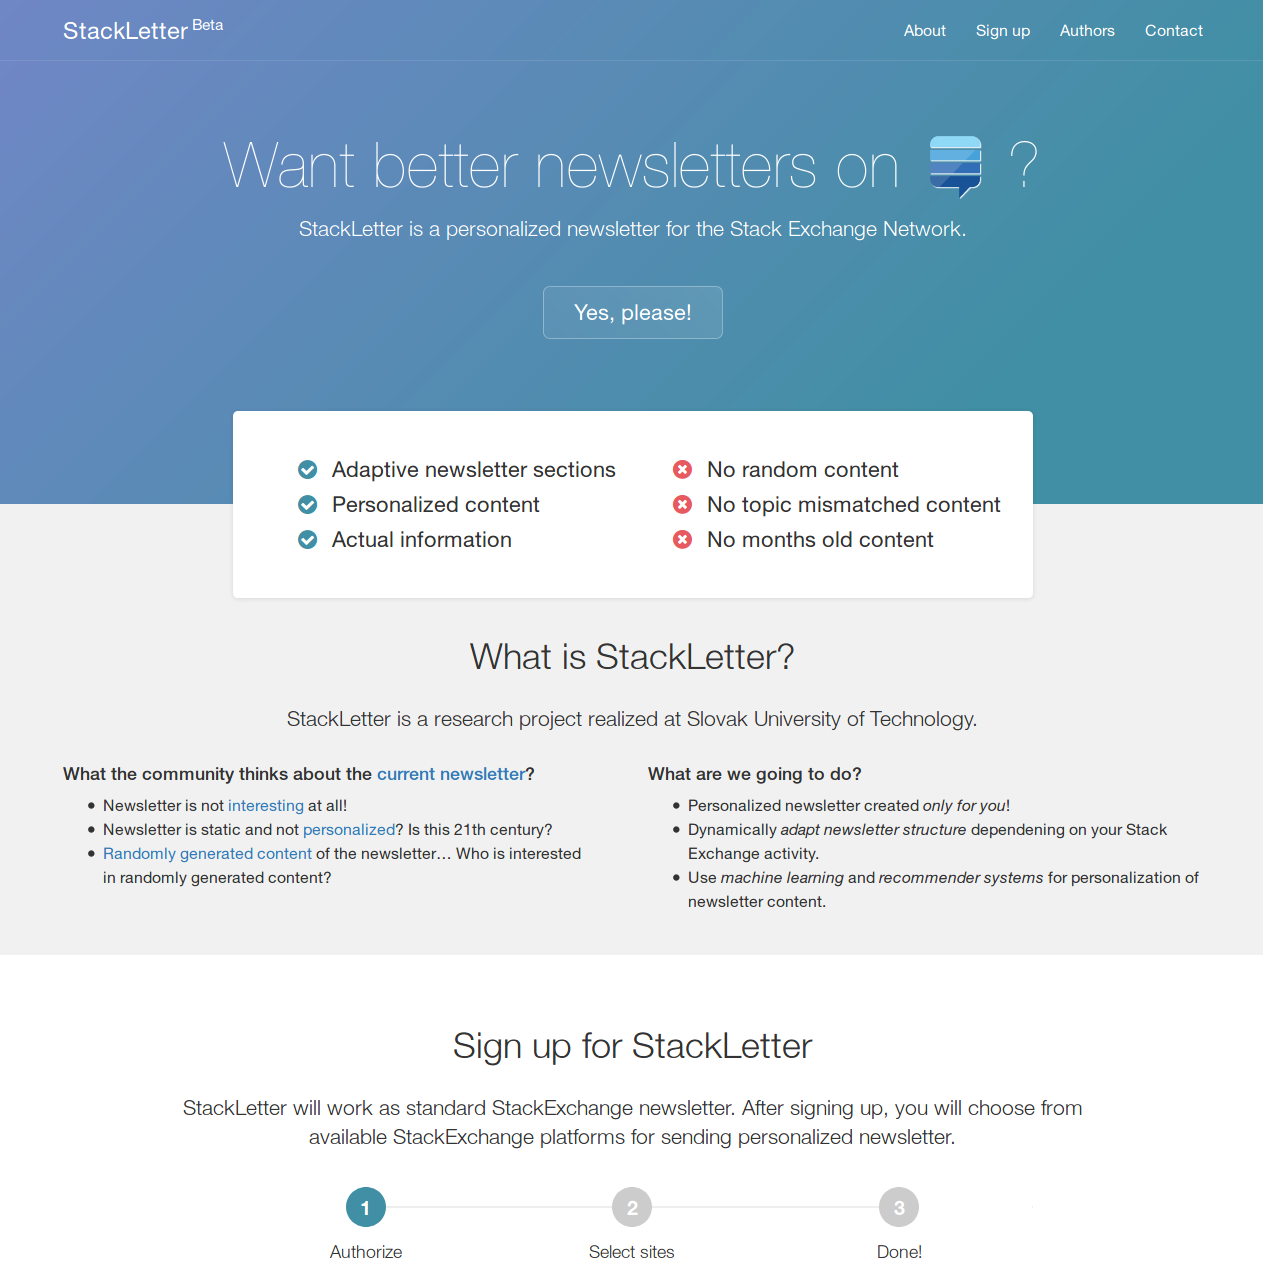
\includegraphics[scale=0.25]{stackletter-screenshot}
\caption{Snímka registračnej stránky StackLetter.com. \label{fig:stackletter.com}}\end{center}
\end{figure}

\textbf{Modul pre generovanie a odosielanie informačných bulletinov}\\
Tento modul je zodpovedný za samotné zostavovanie a odosielanie informačných bulletinov jednotlivým zaregistrovaným
používateľom. Prostredníctvom REST API komunikuje s modulmi pre zostavovanie odporúčaní a štruktúry informačných bulletinov
a na základe ich odpovedí vygeneruje naformátované informačné bulletiny, ktoré sú následne rozosielané prostredníctvom služby
SendGrid\footnote{\url{https://sendgrid.com}}.

\textbf{Modul pre spracovanie statickej zálohy databázy}\\
Modul bol navrhnutý a implementovaný za účelom rýchleho a efektívneho importovania počiatočných dát platformy Stack Exchange
dostupných vo forme XML exportu do našej internej reprezentácie v databáze PostgreSQL.

Podrobný technický a architektonický popis jednotlivých modulov sa nachádza
v prílohe~\ref{tech-doc} -- \textit{Technická dokumentácia systému StackLetter}.

\section{Použité technológie a služby}

\begin{my_itemize}
\item{Jednotlivé moduly zabezpečujúce infraštruktúru systému StackLetter sú implementované v~jazyku PHP\footnote{\url{https://php.net}}
verzie~7.1 s použitím MVC frameworku Nette~2.4\footnote{\url{https://nette.org}}.}
\item{Systém na ukladanie dát využíva relačný databázový systém PostgreSQL vo verzii 9.6 a vnútropamäťové dátové úložisko Redis
vo verzii 4.0.}
\item{Systém komunikuje s platformou Stack Exchange prostredníctvom Stack Exchange API v2.2 a~vykonáva autentifikáciu
používateľov prostredníctvom protokolu OAuth 2.0.}
\item{Na hromadné odosielanie informačných bulletinov používateľom prostredníctovm e-mailu je využitá služba SendGrid.}
\item{Modul implementujúci zostavovanie personalizovaných informačných bulletinov so zameraním na diverzitu bude implementovaný
v jazyku Python 3.6.}
\end{my_itemize}



\chapter{Experimentálne overenie}


\section{Návrh overenia metód}

Nami navrhnuté metódy personalizovaného odporúčania a diverzifikácie odporúčaného obsahu budeme overovať prostredníctvom
online nekontrolovaného experimentu spoločne s kolegom Matúšom Salátom~\cite{Salat2018} na používateľoch z komunity \textit{Stack Overflow} platformy Stack Exchange.

Tento online experiment bude mať formu pravidelne rozposielaného informačného bulletinu, na ktorého odoberanie sa budú
môcť prihlásiť všetci používatelia z tejto komunity.

Účinnosť zvolených metód diverzifikácie odporúčaní budeme vyhodnocovať prostredníctvom A/B testovania, pričom používateľov
rozdelíme na štyri skupiny:
\begin{my_enumerate}
    \item{Kontrolná skupina -- generický informačný bulletin bez odporúčania;}
    \item{Skupina A -- informačný bulletin s odporúčaním, bez diverzifikácie;}
    \item{Skupina B -- informačný bulletin s odporúčaním, metóda proporčnej diverzifikácie;}
    \item{Skupina C -- informačný bulletin s odporúčaním, metóda tématického vzorkovania;}
\end{my_enumerate}

Dôležitým predpokladom pre úspešnosť online experimentu bude získať dostatočnú reprezentatívnu vzorku používateľov
ochotných byť súčasťou experimentu. V~prípade, že by sa nám nepodarilo osloviť dostatočný počet používateľov, plánujeme
vykonať kontrolovaný offline experiment na vzorke archívnych dát.


\section{Metriky hodnotenia výsledkov}

Pre overovanie výsledkov experimentov budeme používať tieto metriky:

\textbf{Precision@N}\\
Presnosť (angl.~\emph{Precision}), alebo tiež \textit{pozitívna predikčná hodnota} je metrika reprezentujúca pomer relevantných
dokumentov z celkového zoznamu. Štandardne sa presnosť počíta ako pomer z celého zoznamu dokumentov, no v oblasti
odporúčania a vyhľadávania informácií je často vhodnejšou odvodená metrika \textit{Precision@N}, ktorá určuje, aká časť
z prvých N dokumentov v zozname je relevantná.
$$\mbox{Precision@N}=\frac{|\{\mbox{relevantne otazky v top-N}\}\cap\{\mbox{top-N odporucenych otazok}\}|}{|\{\mbox{top-N odporucenych otazok}\}|}$$

\textbf{nDCG}\\
\textit{Normalized Discounted Cumulative Gain} je metrika kvality ohodnocovania často používaná na meranie efektívnosti
odporúčania. DCG meria užitočnosť dokumentov na základe ich pozície vo výslednom zozname. Užitočnosť dokumentov sa akumuluje
od konca zoznamu, pričom najvyššiu užitočnosť majú dokumenty na začiatku zoznamu~\cite{Jrvelin2002}.

nDCG položky na pozícii $p$ v zozname odporúčaní je definované ako:

$$\mathrm{nDCG_{p}} = \frac{DCG_{p}}{IDCG_{p}}$$
$$\mathrm{DCG_{p}} = \sum_{i=1}^{p} \frac{ 2^{rel_{i}} - 1 }{ \log_{2}(i+1)}$$
$$\mathrm{IDCG_{p}} = \sum_{i=1}^{|REL|} \frac{ 2^{rel_{i}} - 1 }{ \log_{2}(i+1)}$$
\begin{adjustwidth}{1cm}{1cm}
$rel_i$ -- relevancia $i$-tej položky v zozname odporúčaní.\\
$|REL|$ -- zoznam $p$ relevantných položiek zo zoznamu odporúčaní usporiadaných podľa relevancie.
\end{adjustwidth}

\textbf{CTR}\\
Miera preklikov (angl.~\emph{Click-through Rate}) je metrika často využívaná v spojitosti s informačnými bulletinmi.
Táto metrika vyjadruje počet úspešných kliknutí na odkaz v informačnom bulletine.

Okrem CTR plánujeme v súvislosti s interakciou používateľa s informačným bulletinom merať aj počet impresií,
teda zobrazení informačného bulletinu, ako aj počet konverzií, teda podiel prípadov, kedy kliknutie na niektorú z otázok
v informačnom bulletine viedlo k aktivite používateľa na tejto otázke -- či už označenie za obľúbenú,
odpovedanie alebo pridanie komentáru. Ďalej tiež plánujeme merať počet odhlásení z informačného bulletinu.


%%
%% results
%%
%!TEX root = main.tex
\newpage
\ifthenelse {\boolean{bachelor}}
{
	\section{Results}
	%\section{Výsledky}
}
{
	\chapter{Results}
	%\chapter{Výsledky}
}
Lorem ipsum dolor sit amet, consectetuer adipiscing elit, sed diam nonummy nibh euismod tincidunt ut laoreet dolore magna aliquam erat volutpat. Ut wisi enim ad minim veniam, quis nostrud exerci tation ullamcorper suscipit lobortis nisl ut aliquip ex ea commodo consequat.

\ifthenelse {\boolean{bachelor}}
{
	\subsection{Subsection}
	%\subsection{Podčasť}
}
{
	\section{Subsection}
	%\section{Podčasť}
}
\label{label}
Lorem ipsum dolor sit amet, consectetuer adipiscing elit, sed diam nonummy nibh euismod tincidunt ut laoreet dolore magna aliquam erat volutpat. Ut wisi enim ad minim veniam, quis nostrud exerci tation ullamcorper suscipit lobortis nisl ut aliquip ex ea commodo consequat. Duis autem vel eum iriure dolor in hendrerit in vulputate velit esse molestie consequat, vel illum dolore eu feugiat nulla facilisis at vero eros et accumsan et iusto odio dignissim qui blandit praesent luptatum zzril delenit augue duis dolore te feugait nulla facilisi. Nam liber tempor cum soluta nobis eleifend option congue nihil imperdiet doming id quod mazim placerat facer possim assum. Typi non habent claritatem insitam; est usus legentis in iis qui facit eorum claritatem. Investigationes demonstraverunt lectores legere me lius quod ii legunt saepius. Claritas est etiam processus dynamicus, qui sequitur mutationem consuetudium lectorum. Mirum est notare quam littera gothica, quam nunc putamus parum claram, anteposuerit litterarum formas humanitatis per seacula quarta decima et quinta decima. Eodem modo typi, qui nunc nobis videntur parum clari, fiant sollemnes in futurum.


%%
%% Conclusion
%%
%!TEX root = main.tex
\newpage

\chapter{Zhodnotenie}

V súčasnosti je systém StackLetter nasadení v testovacej prevádzke. Zatiaľ používateľom umožňuje nechať si odosielať
informačné bulletiny pre komunity \textit{Stack Overflow} a \textit{Software Engineering} buď raz denne, alebo raz týždenne.

\begin{table}[h]
\centering
\caption{Používanosť systému StackLetter}
\begin{tabular}{|m{10cm}|m{1.5cm}|}
\hline
Počet odoberateľov informačného bulletinu & 24 \\ \hline
Počet odoslaných informačných bulletinovu & 493 \\ \hline
Počet používateľmi otvorených informačných bulletinov & 119\footnotemark \\ \hline
Počet otvorených položiek informačných bulletinov & 145 \\ \hline
Počet explicitných hodnotení informačných bulletinov & 114 \\ \hline
\end{tabular}
\end{table}

\footnotetext{Počet otvorení môže byť skreslený, nakoľko viaceré klienty blokujú zobrazenie obrázkov použitých na vyhodnotenie otvorenia e-mailu.}

Obsah informačného bulletinu je zatiaľ personalizovaný len jednoduchou metódou na základe značiek, v ktorých má používateľ aktivitu.
Návrh metód odporúčania s~podporou diverzity a~aktuálnosti je v tejto fáze práce už finalizovaný.

V nasledujúcom semestri plánujeme implementovať metódy odporúčania s~podporou diverzity a~aktuálnosti a ďalej pokračovať
v online nekontrolovanom experimente. V prípade vyhodnotenia tohto experimentu ako neúspešného máme v pláne vykonať
online konktrolovaný experiment. Podrobnejší plán práce v ďalšom semestri obsahuje príloha~\ref{apx:dp3plan}.


%%
%% References
%%
\afterpage{\blankpage}
\newpage
\addcontentsline{toc}{chapter}{\refname}
\bibliographystyle{unsrt}
\bibliography{references.bib}

%%
%% Appendix
%%
\newpage
\ifthenelse {\boolean{bachelor}}
{
}
{
    \ifthenelse {\boolean{english}}
    {
        \renewcommand{\appendixname}{Appendix}
        \renewcommand{\appendixtocname}{Appendix}
    }
    {
        \renewcommand{\appendixname}{Príloha}
        \renewcommand{\appendixtocname}{Prílohy}
    }
    \pagenumbering{bychapter}
}
\appendix
%!TEX root = main.tex
\newpage
\thispagestyle{plain}

\chapter{Plán práce na diplomovom projekte}

\section{Plán práce na diplomovom projekte I}

Prácu na diplomovom projekte I sme navrhli a naplánovali nasledovne:

\begin{table}[h]
\centering
\caption{Plán práce na diplomovom projekte I}
\begin{tabular}{|m{2.3cm}|m{12cm}|}
\hline
1-5.~týždeň semestra   & Analýza problematiky odporúčania v kontexte CQA systémov a súčasného výskumu v tejto oblasti. \\ \hline
6-7.~týždeň semestra   & Analýza dostupných dát na platforme Stack Exchange a možností verejného API platformy. \\ \hline
8-9.~týždeň semestra   & Vytvorenie predbežného návrh metódy riešenia problému a návrh metód overenia výsledkov. \\ \hline
10-12.~týždeň semestra & Spísanie správy diplomového projektu I v rátane analýzy a predbežného návrhu riešenia a overenia. \\ \hline
\end{tabular}
\end{table}

\textbf{Zhodnotenie}\\
Navrhnutý plán práce v rámci diplomového projektu I sa nám do veľkej miery podarilo dodržať. Časový sklz sa prejavil až
vo fáze návrhu metódy riešenia problému, čím sa posunulo spísanie správy až do 11. týždňa semestra.

\newpage
\section{Plán práce na diplomovom projekte II}

\begin{table}[h]
\centering
\caption{Plán práce na diplomovom projekte II}
\begin{tabular}{|m{2.3cm}|m{12cm}|}
\hline
1-2.~týždeň semestra   & -- Príprava databázy a aktualizačného modulu.
				\newline -- Vytvorenie modelov pre získavanie spätnej väzby od používateľov.
				\newline -- Prvotná dátová analýza.
				\\ \hline
3-4.~týždeň semestra   & -- Príprava rozhrania pre odoberanie informačných bulletinov.
				\newline -- Generovanie informačných bulletinov na základe prvotného modelu.
				\newline -- Nasadenie systému a otestovanie v reálnych podmienkach.
				\\ \hline
5-8.~týždeň semestra   & -- Získavanie používateľov informačného bulletinu.
				\newline -- Spracovanie dát, vytvorenie reálnych modelov používateľov a otázok, generovanie odporúčaní.
				\newline -- Príprava metód diverzifikácie odporúčaní.
				\newline -- Písanie diplomovej práce.
				\\ \hline
9-12.~týždeň semestra  & -- Overenie a vyhodnocovanie informačných bulletinov.
				\newline -- Nasadenie a porovnanie metód diverzifikácie.
				\newline -- Počiatočné overenie výsledkov.
				\newline -- V prípade neúspechu online experimentu, plánovanie offline expermientov.
				\\ \hline
\end{tabular}
\end{table}

\section{Plán práce na diplomovom projekte III}

\begin{table}[h]
\centering
\caption{Plán práce na diplomovom projekte III}
\begin{tabular}{|m{2.3cm}|m{12cm}|}
\hline
1. mesiac & Pokračovanie v experimentoch, nasadzovanie systému na väčšom množstve dát. \\ \hline
2. mesiac & Analýza výsledkov experimentov, vyhodnotenie úspešnosti projektu. \\ \hline
3. mesiac & Dokončenie diplomovej práce.\\ \hline
\end{tabular}
\end{table}


\section{Technická dokumentácia systému StackLetter}\label{tech-doc}


\end{document}

%%%%%%%%%%%%%%%%%%%%%%%%%%%%%%%%%%%%%%%%%%%%%%%%%%%%%%%%%%%%%%%%%%%%%%%%%%%%%%%%%%%%%%%%

%%
%% !!!! set your own details
%%
%\begin{comment}
%[x] [Autor Dokumentu], [Nazov Stranky], [URL], [Datum Navstevy]
%\end{comment}
